\section{Technical Implementation and Details}

\subsection{FIDO2}

As already briefly introduced in \autoref{subsec:fido_alliance}, the \gls{fido}2 project is joint efforts of the \gls{w3c} and the \gls{fido} alliance. It consists of the \gls{js} standard, the \wa{}, and the \glsfirst{ctap}. The \wa{} is standardized and managed by the \gls{w3c}, while the \gls{ctap} is authored by the \gls{fido} alliance. However, the \gls{fido} alliance also initially developed the \wa{} under the name \gls{fido} 2.0 before officially handing it over to the \gls{w3c}.\footcites[See][254]{Schwartz2018}[See][3]{FormalVerificationWebAuthn}

\begin{figure}[hbt]
	\centering
	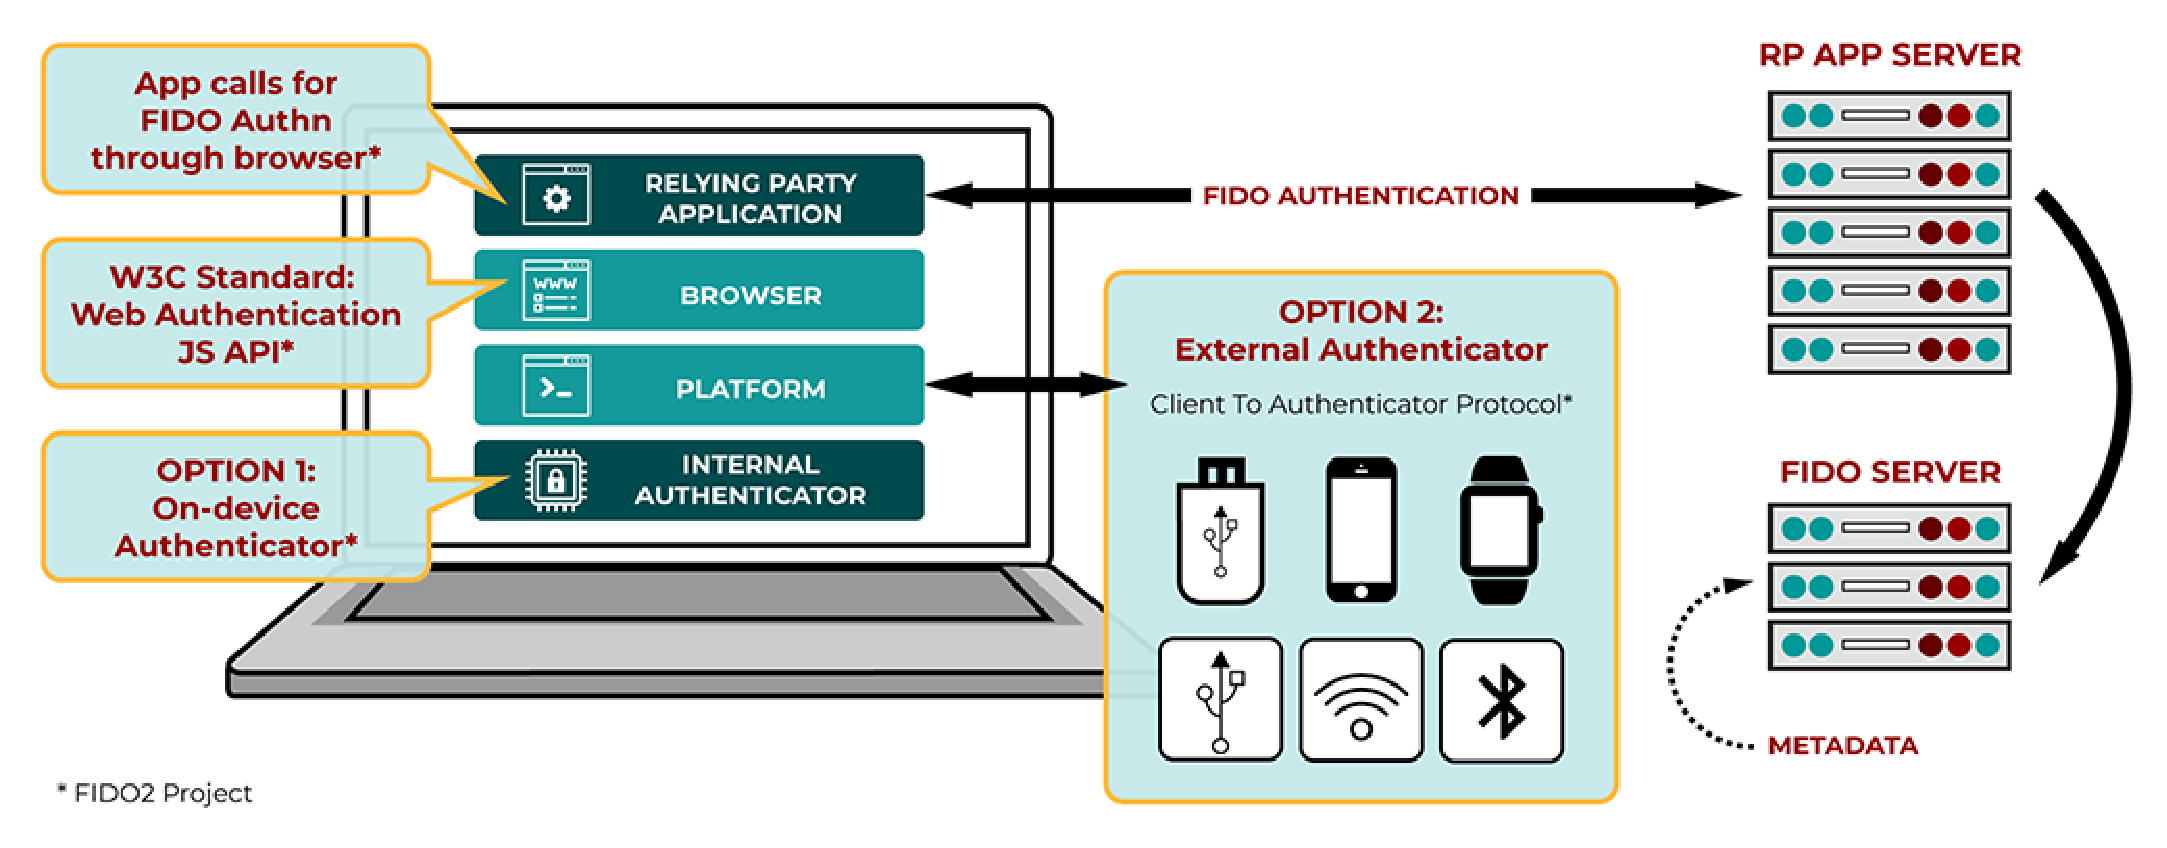
\includegraphics[width=\textwidth]{pics/FIDO2-Graphic-v2.eps}
	\caption[\gls{fido}2 architecture overview]{\gls{fido}2 architecture overview\footnotemark}
	\label{fig:fido2_architecture}
\end{figure}
\footnotetext{Source: https://fidoalliance.org/specifications/, last accessed on 09/14/2019}

\autoref{fig:fido2_architecture} shows the overview of the \gls{fido}2 project. A noteworthy change in contrast to the \gls{u2f} specification is the possibility to use either a \textit{roaming}, i.e., external authenticator or an authenticator that is built into the device or platform, respectively.

\subsection{Client to Authenticator Protocol 2}

The \glsfirst{ctap} 2 is based on the \gls{u2f} protocol version 1.2 and defines three parts:

\begin{enumerate}
	\item the authenticator \gls{api}
	\item message encoding
	\item transport-specific bindings
\end{enumerate}

The key methods of the authenticator \gls{api} are explained in more detail below. Message encoding describes the process of encoding the corresponding message in a binary form called \gls{cbor}. This binary form is suitable for, e.g., the transport over \gls{ble}, because plain text strings and \gls{json} objects can be too big for a transport over low data rate protocols. The transport-specific bindings define the required transformation and bindings in order to comply with the transport protocol specifications.\footcites[See][4--5]{ctap2}

An important difference between \gls{ctap}2 and the preceding standard \gls{u2f} is the fact that \gls{ctap}2 describes only the communication between the client, i.e., web browser and the authenticator, as opposed to \gls{u2f} where the standard also defines the \gls{js} \gls{api} in order to communicate with the authenticator. \autoref{fig:ctap_vs_u2f} shows this architectural difference.\footcites[See][51]{kim-new-way-fido}[See][254]{Schwartz2018}

\begin{figure}[hbt]
	\centering
	\includesvg[width=\textwidth,pretex=\relscale{0.8}]{pics/svg/ctap_vs_u2f}
	\caption[Architectural differences between \gls{u2f} and \gls{ctap}2]{Architectural differences between \gls{u2f} and \gls{ctap}2\footnotemark}
	\label{fig:ctap_vs_u2f}
\end{figure}
\footcitetexts[Source: diagram by author, based on][4]{u2f-overview}[][Chapter 6]{w3c}

\newpage

\subsubsection{Registration}

The registration procedure invokes the method \textit{authenticatorMakeCredential}. The input parameters are identical to the ones defined in the higher level \wa{} and are further explained in \autoref{subsec:wa}. Upon reception of the required data, the authenticator first checks if the \textit{excludeList} contains a credential ID that is already registered with the authenticator. This prevents that a user registers multiple accounts for the same \gls{rp}. If the user verification or presence option is passed, the authenticator has to ensure a legitimate user is present. Upon successful user verification the authenticator generates a new credential key-pair for the specified algorithm.\footcites[See][9]{ctap2}

After that, the authenticator generates the attestation object. It consists of the authentication data, which contains the hash of the \gls{rp} ID, a counter, flags if the user has been verified, and the public key with its unique credential ID. Besides that, the authenticator also sends the attestation statement, if required. This statement can for example be issued by the \gls{tpm}, Android Key attestation, or be generated with private attestation key of the authenticator token.\footcites[See][9]{ctap2}[See][Chapter 8]{w3c}

\subsubsection{Authentication and Transaction Confirmation}

Authentication is performed by using the method \textit{authenticatorGetAssertion} of the \gls{ctap}, where the higher level \wa{} defines the input parameters. The identifier of the \gls{rp} is sent to the authenticator and optionally a list of public keys the authenticator is allowed to retrieve. After optional user verification and presence detection, the authenticator displays the data to the user if it has a display to do so. When these checks succeeded, the authenticator accesses the corresponding credential.\footcites[See][11-13]{ctap2}

The authenticator generates an assertion signature over the received hash of the client data and the authenticator data. The authenticator data consist of the hashed \gls{rp} ID, the flags for user presence and verification, a counter, and the attested credential data. The attested credential data comprises the \gls{aaguid}, credential ID, and the credential public key.\footcites[See][Chapter 6.4.1.]{w3c}

\subsubsection{Factory Reset}

As the \gls{uaf} protocol, but in contrast to the \gls{u2f} specification, the \gls{ctap} defines a method to completely factory reset the authenticator in order to de-register every user account and key material stored on it. To avoid accidental deletion of all user accounts, the protocol specifies that the authenticator may ask for user confirmation. However, it is not possible to delete a specific user account and key-pair.\footcites[See][26]{ctap2}

\subsection{Web Authentication API}
\label{subsec:wa}

The \gls{api} defined in the \wa{} is actually an extension of the Credential Management \gls{api}. This is another \gls{api} in development by the \gls{w3c}, but currently in a draft state and not a recommendation yet.\footnote{The \gls{w3c} standardization process can be viewed in the \autoref{sec:w3c-process}} The Credential Management \gls{api} defines the \textit{navigator.credentials} property with the \textit{create} and \textit{get} methods. Its the goal is to offer an \gls{api} for programmatically accessing the user agent's password storage capabilities. The \wa{} is adding further method overloads to support public-key based credentials, too.\footcites[See][Chapter 1]{w3c}[See][Chapter 1.1]{w3c-credentials}

Authentication and registration in the context of the \wa{} are a special form of network protocols, called a \textit{ceremony}. A ceremony describes the concept of extending a network protocol to include human nodes, too. This allows the specification to take the human factor into account, too.\footcite[See][2]{Ellison2007CeremonyDA}

The \wa{} is backwards compatible to the \gls{u2f} protocol, thus making every security token that is usable for \gls{u2f} compatible with the \wa, too. However, a crucial restriction of the legacy \gls{u2f} protocol in usage with \gls{fido}2 is that it is only usable as a second factor and not for passwordless logins.\footcites[See][Chapter 2.2.1, 6.1.2]{w3c}

\subsubsection{Registration}

A new key-pair for the registration with a \gls{rp} is generated when the client invokes the asynchronous method \textit{navigator.credentials.create} with an object that contains the required \textit{publicKey} property. The publicKey object contains the ID, name of the \gls{rp}, and the user information consisting of a username, display name, and a unique ID. Given the fact that, e.g., the authenticator stores the ID value, it should not consist of any information that can be linked to the user. Further, the publicKey object contains a random challenge generated by server to prevent replay attacks.\footcites[See][Chapter 5.1.3]{w3c}

Besides that, with the public key credential parameters array (\textit{pubKeyCredParams}) it is possible for the \gls{rp} to define the desired algorithm that should be used for the key-pair generation. The algorithm (\textit{alg}) IDs are obtained from the \gls{iana} registry of \gls{cose} algorithms. The ID -7 expands to \gls{ecdsa} with \gls{sha}-256, while -257 links to the \gls{rsa} algorithm in conjunction with \gls{sha}-256. The order in the array describes the preferred algorithm, but also accepted fallback algorithms.\footcites[See][Chapter 5.3, 11.3]{w3c}

Additionally, the \gls{rp} can define a list of credentials (\textit{excludeCredentials}) that need to be check if they exist, e.g., prevent the user from creating multiple key-pairs for the same \gls{rp}. Furthermore a \textit{timeout} value can be specified in which the operation should succeed or fail.\footcites[See][Chapter 5.4]{w3c}

Moreover, the \gls{rp} can set the \textit{authenticatorSelection} property which defines the requirement if a user needs to be verified (possible values are \textit{required}, \textit{preferred}, \textit{discouraged}), the option if the credentials need to be stored on the authenticator (\textit{requireResidentKey}). Further, the \gls{rp} can specify the authenticator attachment modality, i.e., if the authenticator should be platform specific or a cross-platform (roaming) authenticator.\footcites[See][Chapter 6.2.1]{w3c}

Finally, the \textit{attestation} property is of importance. The \gls{rp} can specify either a \textit{direct}, \textit{indirect}, or \textit{none} attestation. None means that the \gls{rp} is not interested in the attestation of the authenticator at all. A direct attestation requires a signed attestation statement generated by the authenticator to verify its authenticity. In contrast, an indirect attestation leaves the authenticator in charge how to generate the attestation certificate. The authenticator may use a per-origin \gls{ca} to protect the users privacy or implement and use the \gls{ecdsa}.\footcites[See][Chapter 5.4.6]{w3c}

\begin{example}{Exemplary Web Authentication API registration}{listing:webauthnreg}
\begin{minted}[breaklines]{javascript}
const publicKeyOptions = {
  challenge: 'Wings2019', // normally a random string from the server in binary form (Uint8Array)
  rp: {
    name: 'Web Authn Test',
    id: 'https://timbrust.de'
  },
  user: {
    id: 'C0E3F2BFCFA8179F', // usually in binary form (Uint8Array)
    name: 'me@timbrust.de',
    displayName: 'tim'
  },
  pubKeyCredParams: [{ alg: -7, type: 'public-key' }],
  authenticatorSelection: {
    authenticatorAttachment: 'cross-platform'
  },
  timeout: 600,
  attestation: 'none'
};

const credential = await navigator.credentials.create({
  publicKey: publicKeyOptions
});
\end{minted}
\end{example}

\autoref{listing:webauthnreg} shows an example payload for the registration of a new credential with the \wa{} consisting of the previously introduced parameters. The \textit{publicKeyOptions} payload generated and sent by the \gls{rp} can be passed to the authenticator by calling the \gls{ctap} \textit{authenticatorMakeCredential} method. The client passes the user and \gls{rp} to the authenticator. Further, it is evaluated if the authenticator should verify the user or if a check of user presence is sufficient. For this evaluation the property \textit{userVerification} is used. Besides that, the list of credentials to exclude, the public key credential parameters and the hash of the client data is provided to the authenticator. The client data comprises the server provided challenge, it's origin and the string type \textit{webauthn.create}.\footcites[See][Chapter 5.4, 6.4.2]{w3c}

Upon reception of the \textit{attestationObject} from the authenticator, the client can generate the credential to be returned to the \gls{rp}, as shown in \autoref{listing:webauthnregresp}.
\\
\begin{example}{Web Authentication API registration response}{listing:webauthnregresp}
\begin{minted}[breaklines]{javascript}
const credential = {
  id: 'BShOCQ2c32dv4aqyy3oWmcu_9s4tz0VIob81U5tg [...]',
  rawId: ArrayBuffer(59),
  response: {
    clientDataJSON: ArrayBuffer(121),
    attestationObject: ArrayBuffer(306)
  },
  type: 'public-key'
};
\end{minted}
\end{example}

The created \textit{credential} object consists of an \textit{ID}, both as a string and binary representation, the \textit{type} that is always set to \frqq public-key\flqq{} and the \textit{response} object. The response object is constructed from the returned \textit{attestationObject} and the client data, which is also shown in \autoref{listing:webauthnregrespclientdata}.\footcite[See][Chapter 5.1]{w3c}
\\
\begin{example}{Web Authentication API registration client data}{listing:webauthnregrespclientdata}
\begin{minted}[breaklines]{javascript}
const clientDataJSON = {
  challenge: 'Wings2019',
  origin: 'https://timbrust.de',
  type: 'webauthn.create'
};
\end{minted}
\end{example}

\autoref{listing:webauthnregrespclientdata} shows the decoded client data from the \wa{} registration response from \autoref{listing:webauthnreg}. The data contains the \textit{challenge} sent by the \gls{rp} and the \textit{origin} of the \gls{rp}. Each registration is flagged with the \textit{type} of \frqq webauthn.create\flqq.\footcites[See][Chapter 5.10.1]{w3c}

In contrast, the \textit{attestationObject} sent from the authenticator contains more properties and is shown in \autoref{listing:webauthnregrespattestation} on the next page. On the first hierarchy it contains the attestation statement format identifier (\textit{fmt}), such as \frqq packed, tpm, or fido-u2f\flqq, the attestation statement (\textit{attmStmt}), and the authentication data (\textit{authData}). The authentication data includes the evaluated user flags, for instance if the user was present or verified, a signature counter, if supported by the authenticator, and the hash of the \gls{rp} ID. In detail, the attested credential data of the authentication data contains the public key ID, the public key itself, e.g., the point on an \gls{ec} and the \gls{aaguid} if attestation is not set to none. Otherwise it is set to 16 zero bytes.\footcites[See][Chapter 5.1.3, 6.1]{w3c}

\begin{example}{Web Authentication API registration attestation}{listing:webauthnregrespattestation}
\begin{minted}[breaklines]{javascript}
const attestationObject = {
  fmt: 'fido-u2f',
  attStmt: {
    sig: '[...]',
    x5c: []
  },
  authData: {
    rpIdHash: '068a7ad7f858dadbf691af6f2f7ca86d4dee5a080b [...]',
    flags: {
      userPresent: true,
      reserved1: false,
      userVerified: false,
      reserved2: '0',
      attestedCredentialData: true,
      extensionDataIncluded: false
    },
    signCount: 0,
    attestedCredentialData: {
      aaguid: '0000000000000000',
      credentialIdLength: 96,
      credentialId: ArrayBuffer(59), // identical to publicKeyCredential.id
      credentialPublicKey: {
        kty: 'EC',
        alg: 'ECDSA_w_SHA256',
        crv: 'P-256',
        x: 'xHxgcBFgJolQ5lvukADki+cUzTPcmk50tfj0YGH3nYE=',
        y: 'W1OKIxfc6pIE/ANeTD7MqnNVjBXd0L7We9xZ3Hx6nD8='
      }
    }
  }
};
\end{minted}
\end{example}

\subsubsection{Authentication}

An authentication ceremony is started by calling the client's asynchronous method \textit{navigator.credentials.get}. As in the registration procedure, the \gls{rp} needs to generate a \textit{publicKeyOptions} object. For the authentication a random challenge, a timeout value and the allowed credentials array are required. The \gls{rp} can send a list which associated credentials are suitable for the user assertion. The \gls{rp} may provide an \textit{rpId} and flag for \textit{user verification}, too. If omitted the origin of the \gls{rp} and a default of preferred user authentication is used instead. Each allowed credentials is identified by its id and an optional array of transports the client is allowed to perform to retrieve the credential. \autoref{listing:webauthnauth} on the next page shows the example payload for the assertion.\footcites[See][Chapter 5.1.4., 5.5, 5.10.3.]{w3c}

Subsequently, the user agents generate the \textit{client data} consisting of the origin, challenge, and the type that is always set to \textit{webauthn.get}. It passes the has of the client data, the ID of \gls{rp}, user presence and verification flags, and list of allowed credentials to the authenticator by calling its \textit{authenticatorGetAssertion} method.\footcites[See][Chapter 6.3.3]{w3c}
\\
\begin{example}{Exemplary Web Authentication API authentication}{listing:webauthnauth}
\begin{minted}[breaklines]{javascript}
const publicKeyOptions = {
  challenge: 'Wings2019Auth', // normally a random string from the server in binary form (Uint8Array)
  allowCredentials: [
    {
      id: 'BShOCQ2c32dv4aqyy3oWmcu_9s4tz0VIob81U5tg [...]',
      type: 'public-key',
      transports: ['usb', 'ble', 'nfc']
    }
  ],
  timeout: 6000
};

const assertion = await navigator.credentials.get({
  publicKey: publicKeyOptions
});
\end{minted}
\end{example}

Upon reception of a response from the authenticator, the client can generate the response, i.e., \textit{assertion} object. \autoref{listing:webauthnauthresp} on the next page shows the response that can be sent to the \gls{rp}. The response is similar to a registration response and also contains the credential ID in binary and string representation. Further, the client data is returned to the \gls{rp}, too. The authenticator data is equal to the registration procedure. The most important property is the returned \textit{signature} value over the authenticator data and the client data hash. The \gls{rp} can cryptographically verify the signature with the corresponding public key of the user.\footcites[See][Chapter 5.1.4.1, 5.2.2, 6.3.3]{w3c}
\\
\begin{example}{Web Authentication API authentication response}{listing:webauthnauthresp}
\begin{minted}[breaklines]{javascript}
const assertion = {
  id: 'BShOCQ2c32dv4aqyy3oWmcu_9s4tz0VIob81U5tg [...]',
  rawId: ArrayBuffer(59),
  response: {
    authenticatorData: ArrayBuffer(191),
    signature: ArrayBuffer(59),
    clientDataJSON: {
      challenge: 'Wings2019 Auth',
      origin: 'https://timbrust.de',
      type: 'webauthn.get'
    }
  },
  type: 'public-key'
};
\end{minted}
\end{example}
